\title{\vspace{160px} \textbf{\huge{Multimedia}} \\\vspace{17.5px} \LARGE{Homework 1}  \vspace{10px}}
\author{\href{https://github.com/imAlessas}{Alessandro Trigolo}}
\date{30 Aprile 2024}

\begin{document}

\maketitle\newpage

\tableofcontents\newpage

\listoftodos\newpage


\section{Obiettivo}
\todo{Descrivi decentemente l'obiettivo}



\vspace{30px}\section{Codice sorgente}
\todo{Rifai introduzione}
Il linguaggio scelto per completare le richieste dell'homework è \texttt{Python}; all'interno del documento saranno presenti solo i punti salienti dello script, che comunque può essere ispezionato al seguente \href{https://github.com/imAlessas/computer-networks/blob/main/multimedia/hw-1/script/lossless_coding.py}{\texttt{link}}.



\vspace{15px}\subsection{Entropia dell'immagine}

La prima richiesta dell'homework era divisa in due macro parti, la prima era quella di selezionare e mostrare un'immagine mentre la seconda richiesta chiedeva di calcolare l'entropia dell'immagine.

L'immagine scelta è un'immagine di \textsl{Spider-Man} a colori, di conseguenza è necessario estrarne la luminaza per fara diventare in binaco e nero. Dopo aver caricato l'immagine a colori con l'opportuna funzione \texttt{imread} del pacchetto \texttt{matplotlib.image} è necessario usare la funzione \texttt{cvtColor} del pacchetto \texttt{cv2} di \texttt{opencv}. Il seguente script, dopo aver eseguito le suddette operazioni si occupa di mostrare le due immagini a schermo attraverso una \texttt{subplot}.

\begin{lstlisting}
# Prepare to load the image
img_file_name = "spiderman"
img_extension = ".jpg"
current_dir = os.getcwd()

# path to reach the img
path_to_img = os.path.join(current_dir, "multimedia", "hw-1", "script", "imgs") + "/"

# loads the colored image
img = mpimg.imread(path_to_img +  img_file_name + img_extension) 

# extracts the luminance
gray_img = cv2.cvtColor(img, cv2.COLOR_BGR2GRAY)

# creates a figure with two subplots
fig, axs = plt.subplots(1, 2, figsize=(12, 6))

# displays the colored image in the first subplot
axs[0].imshow(img, cmap='gray')
axs[0].set_title('Colored image')
axs[0].axis('off')

# displays the grayscale image in the second subplot
axs[1].imshow(gray_img, cmap='gray')
axs[1].set_title('Grayscale image')
axs[1].axis('off')
\end{lstlisting}

\noindent Dopo aver eseguito lo script soprastante si può notare che la luminanza dell'immgine è stata estratta con successo (figura \ref{fig:luminanza}).

\begin{figure}[h]
    \centering
    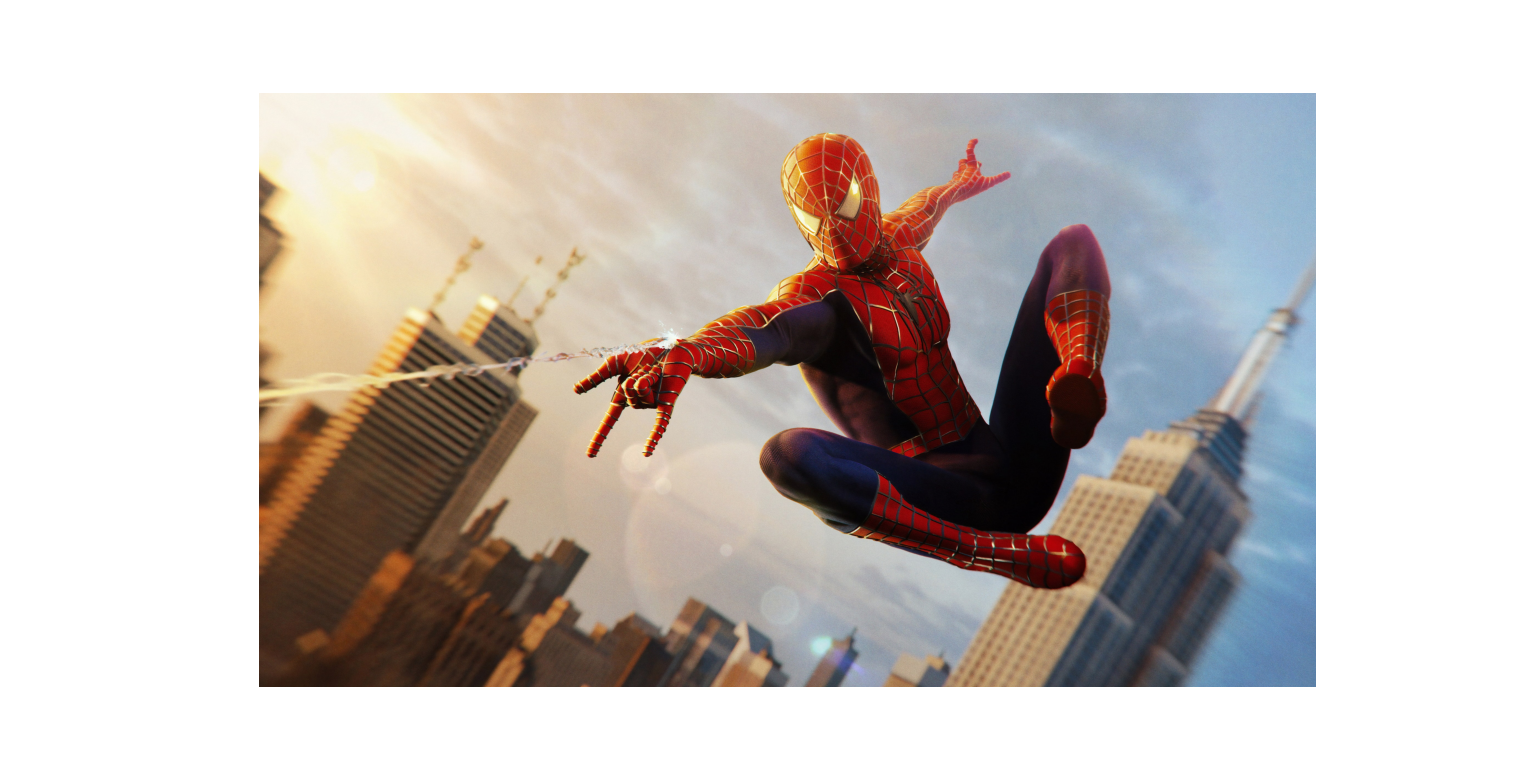
\includegraphics[width = .7\textwidth]{hw-1/report/imgs/colored.png}
    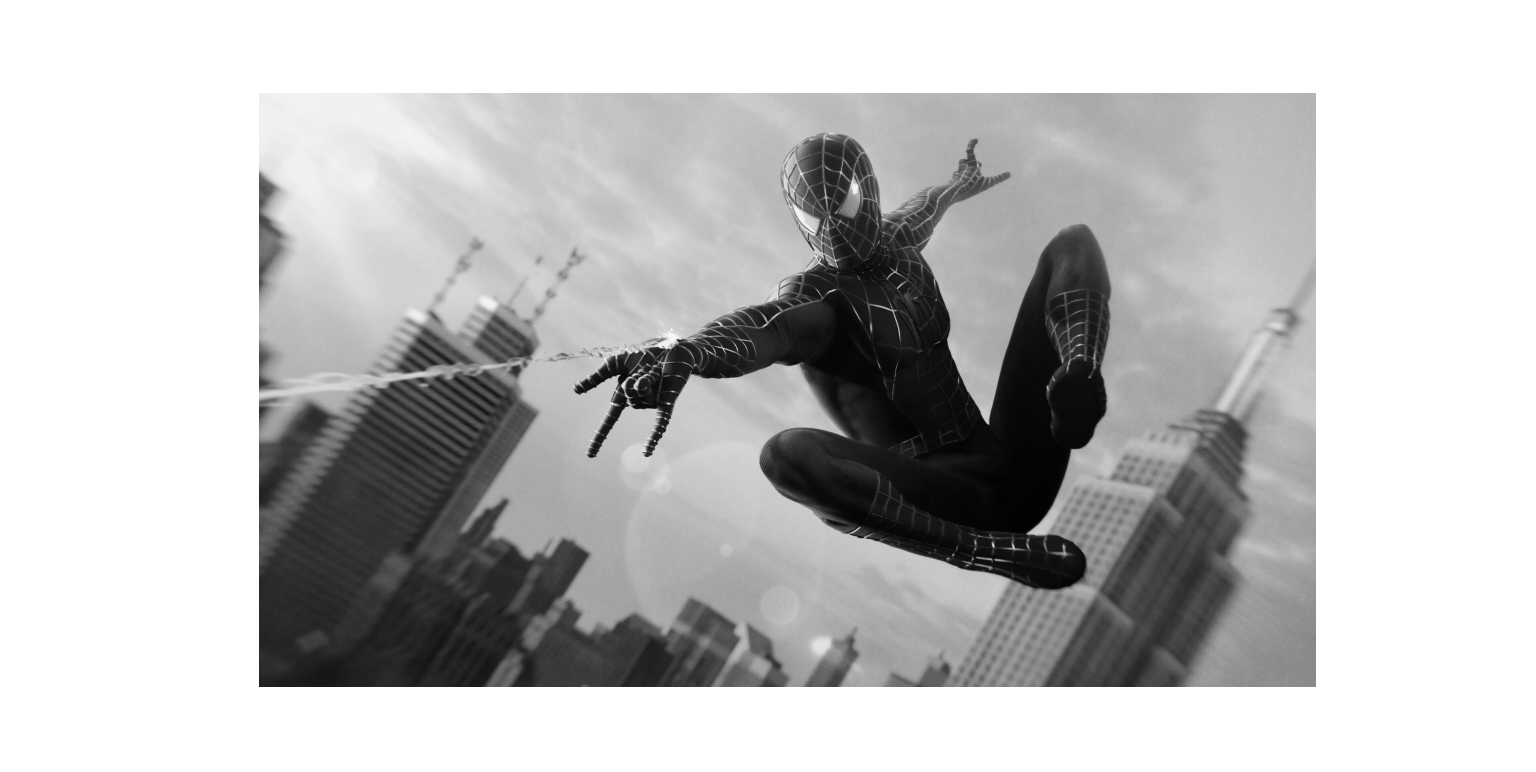
\includegraphics[width = .7\textwidth]{hw-1/report/imgs/grayscale.png}
    \caption{Estrazione della luminaza da una immagine a colori.}
    \label{fig:luminanza}
\end{figure}

\FloatBarrier\noindent In secondo luogo è necessario calcolare l'entropia dell'immagine in bianco e nero. L'entropia di una variabile aleatoria $X$ (in questo caso l'immagine) è definita come l'\textbf{informazione media} degli eventi della sorgente; l'informazione di un evento è descritta dalla funzione seguente:

\begin{gather*}
    I(X) = \log_2\left( \frac{1}{p_i} \right)
\end{gather*}

\noindent Che è una variabile che diminuisce all'aumentare della probabilità dellevento $p_i$. QUuesto è ragionevole in quanto più un evento è imporbabile (quindi $p_i \to 0$) e più la sua informazione è alta ($I(X) \to +\infty$). Assumento che gli eventi della sorgente siano indipendenti, l'informazione media si traduce nella seguente sommatoria:

\begin{gather*}
    H(X) = E[I(X)] \, = \, \sum_{i = 1}^M p_i\log_2\left( \frac{1}{p_i} \right)
\end{gather*}

\noindent Dove con $M$ si indica il numero di elementi nell'insieme $X$. Questa formula si riassume nel seguente script, dove l'immagine viene trasposta e convertita in un vettore di pixel monodimensionale. In secondo luogo attraverso la funzione \texttt{numpy.histogram} vengono contate il numero di occorrenze per ogni valore di pixel. Infine, per calcolare la probabilità, si divide il numero di occorrezze per il numero totale di occorrenze, escludendo eventuali valori diversi da zero.


\begin{lstlisting}
# flatten the transposed matrix to read pixels row by row
rasterScan = np.transpose(gray_img).flatten()

# count the occurrences of each pixel value
occurrencies = np.histogram(rasterScan, bins=range(256))[0]

# calculate the relative frequencies
rel_freq = occurrencies / np.sum(occurrencies)

# remove zero-values of probability
p = rel_freq[rel_freq > 0]

# compute and display the entropy
HX = - np.sum(p * np.log2(p))
print(f"\nThe entropy of {img_file_name} is {HX:.3f} bpp\n")
\end{lstlisting}

\noindent Dopo aver eseguito lo script si ottiene che l'entropia dell'immagine scelta è di circa \textbf{7.530 bpp}.





\vspace{15px}\subsection{Codifica con dizionario}
La seconda task richiedeva di utilizzare una compressione a dizionario, come \texttt{zip} nel caso di \textsl{Windows} per poi calcolare il bitrate risultante. Lo script necessario per soddisfare la richiesta è presentato nel frammento di codice sottostante. In particolare le prime due righe si occupano di \textsl{zippare} il file mentre le seguenti si occupano di ottenere la dimensione dell'immagine compressa. Infine nelle ultime righe si calcola l'effettivo \textsl{bitrate} dividendo la dimensione del file compresso con la dimensione dell'immagine originale, ottenuta mediante l'attrobuto \texttt{size}.

\begin{lstlisting}
# zip the image
cmd = f"zip {path_to_img}{img_file_name}.zip {path_to_img}{img_file_name}.jpg"
os.system(cmd)

# get the zip bytes
img_stats = os.stat(f"{path_to_img}{img_file_name}.jpg")
zip_bytes = img_stats.st_size

# get img size
height, width, _ = img.shape

# get the birate
zip_bitrate = zip_bytes * 8 / (height * width) 

print(f"\nThe bitrate of {img_file_name}.zip is {zip_bitrate:.3f} bpp\n")
\end{lstlisting}

\noindent Dopo aver eseguito lo script si ottiene quindi il valore del bitrate che corrisponde a \textbf{1.340 bpp}, che è molto più basso al valore dell'entropia $H(X)$ osservato nel punto precedente.





\vspace{15px}\subsection{Discussione risultati parziali}
\todo{completa in base al risultato della 2}





\vspace{15px}\subsection{Codifica semplice}
La quarta richiesta dell'homework è quella di effettuare una codifica predittiva \textsl{semplice}. In altre parole, 

\begin{lstlisting}
# calculate prediction error
pred_err = rasterScan[0] - 128
pred_err = np.append(pred_err, np.diff(rasterScan))

# plot error graph
plt.figure()
plt.imshow(np.transpose(np.reshape(np.abs(pred_err), (width, height))), cmap = 'seismic')
plt.axis('image')
plt.axis('off')
plt.colorbar()
plt.title('Prediction Error Magnitude')
\end{lstlisting}

\noindent Dopo aver eseguito lo script soprastatnte si ottiene un'immagine simile affa figura \ref{fig:simple-coding}. Dall'immagine si può notare che le zone più rosse, ovvero le zone in cui il predittore ha fatto più errori sono le zone dei contorni, come la skyline della città oppure lo stacco tra il personaggio raffigurato e il cielo. Questo perchè il distacco dei colori tra una sezione e l'altra è estremamente differente. D'altro canto, le zone colorate di blu sono le zone dove i colori sono più uniformi, ecco quindi che i palazzi e il cielo sono per lo più dello stesso colore, suggerendo poca entropia. \todo{sistema paragrafo}

\begin{figure}[h]
    \centering
    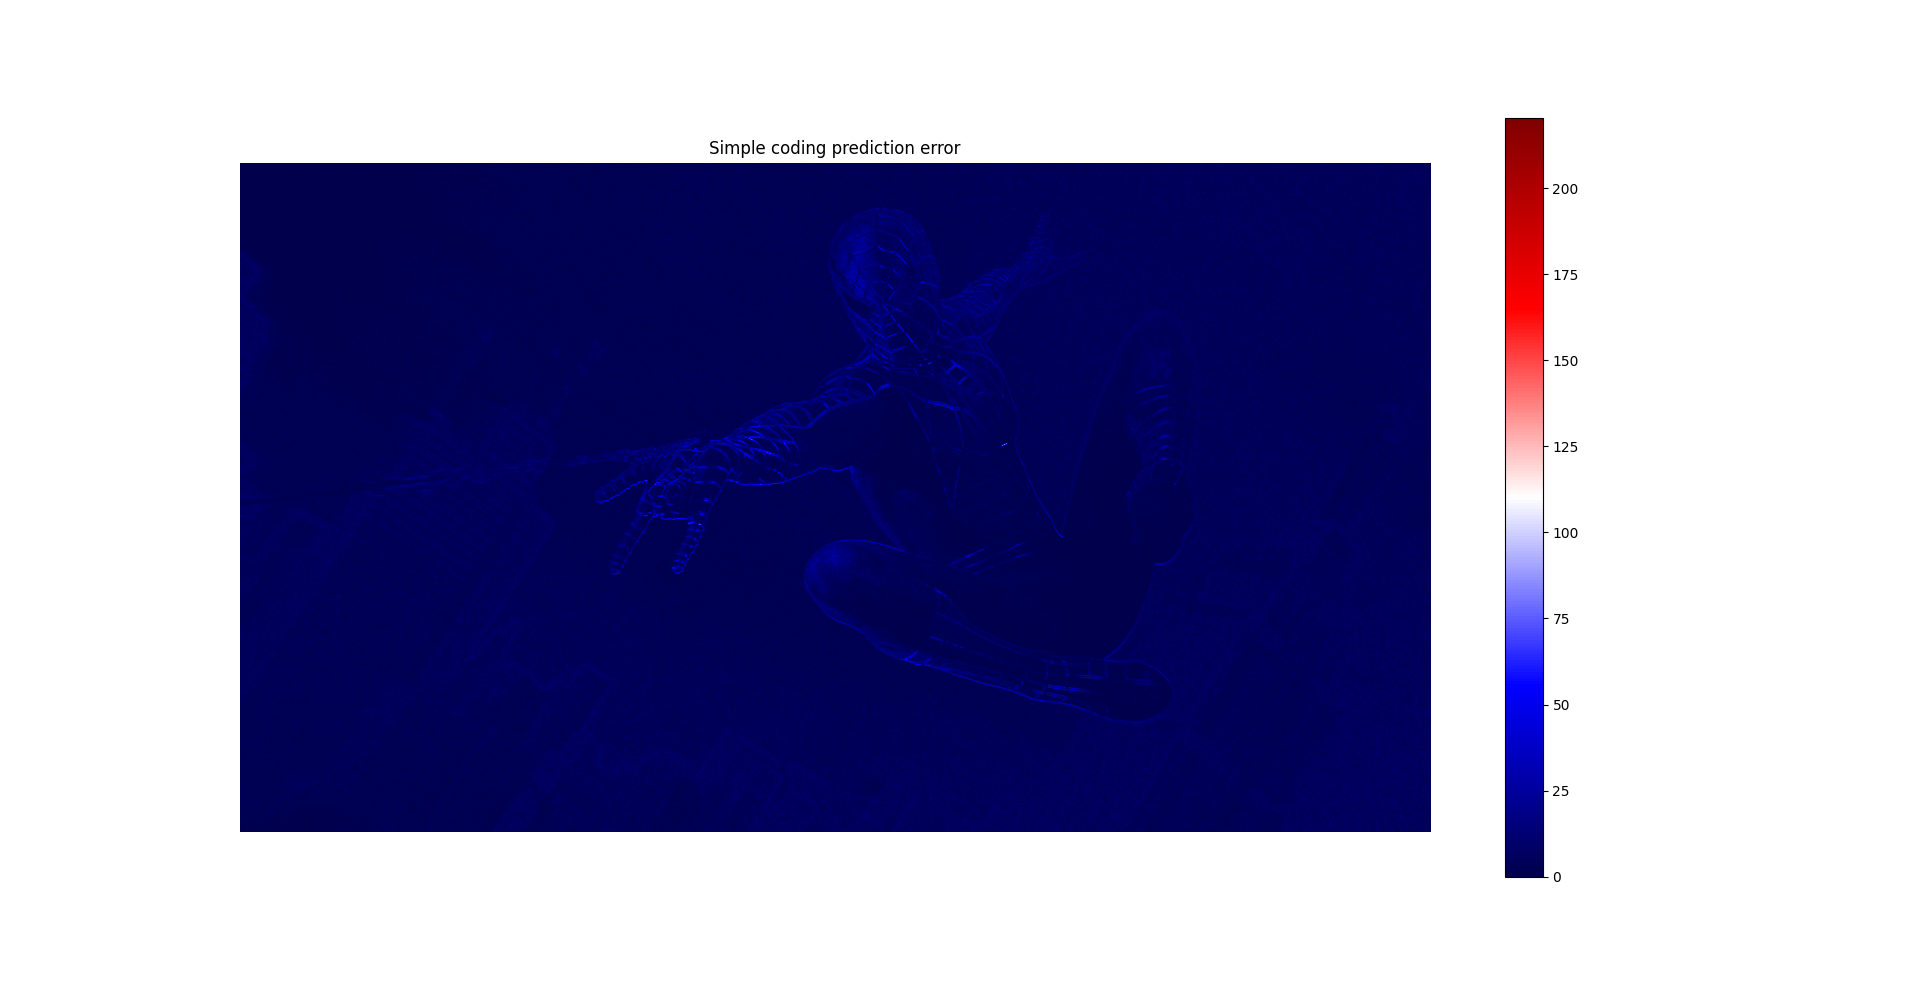
\includegraphics[width = .9\textwidth]{hw-1/report/imgs/simple-coding.png}
    \caption{Rappresentazione del modulo dell'errore di predizione.}
    \label{fig:simple-coding}
\end{figure}

\begin{lstlisting}
# count the occurrences of each prediction error value
occ, _ = np.histogram(pred_err, bins = range(-255, 256))

# calculate the relative frequencies and remove any probability == 0
freqRel = occ / np.sum(occ)
p = freqRel[freqRel > 0]

# calculate the entropy
HY = -np.sum(p * np.log2(1/p))
print(f"The entropy of the prediction error of {img_file_name} is {HY:.3f} bpp")
print(f"The compression ratio of {img_file_name} is {8/HX:.4f}\n")
\end{lstlisting}
\todo{capisci se è da inserire o meno}






\subsubsection{Analisi}





\vspace{15px}\subsection{Codifica avanzata}

prova



\subsubsection{Analisi}





\vspace{30px}\section{Conclusioni}




\end{document}
